% N1 -- Journal of Process Control (Elsevier), regular paper. Plan: N1_OUTLINE.md.
% Build from this folder: pdflatex main, bibtex main, pdflatex main, pdflatex main.
% Figures and generated tables are read from the sibling IPIS checkout
% (IPIS scripts/paper_n1/ writes them to docs/paper/figures/n1/); copy them here only for the
% submission, when the source must be flat.
\documentclass[final,5p,times,twocolumn]{elsarticle}

\usepackage{amsmath,amssymb}
\usepackage{booktabs}
\usepackage{array}
\usepackage{graphicx}
\usepackage{lineno}
\usepackage{url}
\usepackage{tikz}
\usetikzlibrary{arrows.meta,positioning}
\newcommand{\figdir}{../../IPIS/docs/paper/figures/n1}
\graphicspath{{\figdir/}}
% Harmless if unused; pandoc-converted lists need it (IPIS OPEN_ITEMS OI-02).
\providecommand{\tightlist}{\setlength{\itemsep}{0pt}\setlength{\parskip}{0pt}}
\biboptions{sort&compress}
% Two page-wide floats may share a page top, so Figs. 5 and 6 sit beside their first mention.
\renewcommand{\dbltopfraction}{0.85}
\journal{Journal of Process Control}

\begin{document}
\begin{frontmatter}

\title{When the laboratory is late: dead-time analysis and compensation of conformal
soft-sensor intervals}

\author{Bien Don Busico}
\address{University of the Philippines Diliman, Quezon City, Philippines}
\ead{bienbusico@gmail.com}

\begin{abstract}
% 240 words as plain text (the formula as two words, each number with its percent sign as one);
% 249 if every percent sign counts as a word. The journal's limit is 250.
Soft sensors are recalibrated against laboratory or analyzer measurements that arrive late.
Updated with such labels, the single-state recursion of an adaptive conformal interval becomes an
integral loop with dead time: for a delay of $\theta$ updates its linearisation is stable only for
step sizes below $2\sin(\pi/(4\theta+2))$, and on serially correlated residuals it can issue
uninformative intervals while its marginal coverage stays nominal. We test two remedies in a
pre-registered study on 15 Tennessee Eastman runs at three operating points and the debutanizer
data. With the Tennessee Eastman analyzer four updates late, steps tuned without the delay left
6.9\,\% of intervals uninformative, 6.0 percentage points more than without delay, at coverage
0.897. Replaying historical residuals through the delayed loop to tune the step held a 2\,\% budget of uninformative intervals (0.30\,\%). Predicting the persistent
part of the residual and calibrating only the prediction error narrowed the intervals by
18\,\% (95\,\% CI 8 to 28\,\%) at the same budget (0.18\,\%), made misses less persistent and
allowed larger steps; its width was within 1.5\,\% of the best of four conformal PID control
and SPCI configurations. Predicted from the calibration residuals' autocorrelation, the
width ratio erred by $-4.9$\,\% on average at four updates and was conservative at every delay
checked. The delay did not raise the uninformative share on the debutanizer at its primary dead
time, so the diagnosis is restricted to the simulated plant, where compensated split conformal
matched the loop.

\end{abstract}

\begin{keyword}
soft sensor \sep conformal prediction \sep delayed labels \sep dead time \sep
adaptive calibration \sep Tennessee Eastman process
\end{keyword}

\end{frontmatter}

\section{Introduction}\label{sec:intro}

Soft sensors estimate quality variables that are measured slowly, and plants correct them against
laboratory or analyzer values that arrive late \citep{fortuna2007,kadlec2009}: the debutanizer's
gas chromatograph reports about 45~min after sampling \citep[Sec.~6.2]{fortuna2007}, and the
Tennessee Eastman product analyzer after 0.25~h \citep{downs1993}. Soft-sensor research treats
such labels as delayed, infrequent or irregular measurements \citep{guo2014,shardt2016}. An
operator also needs to know how far to trust the estimate, and adaptive conformal inference
\citep{gibbs2021aci} is a natural way to say it: an interval around the prediction whose level is
adjusted online so that a target share of labels falls outside. On a plant, those adjustments can
only use the late labels.

The adjustment is a feedback loop, and the delay puts dead time into it. With the step size tuned
on history that ignores the delay, the loop on the Tennessee Eastman process issued 6.9\,\% of its
intervals uninformative (infinite, or wider than the range of the measured variable) at the
analyzer's documented delay, 6.0 percentage points more than without delay, while the coverage
that is usually reported read 0.897 (Section~\ref{sec:results:diagnosis}). An operator cannot act
on such an interval, and the coverage figure does not show it.

Online conformal methods with delayed feedback exist. Adaptive conformal inference has been run on
labels that arrive several steps late \citep{dixit2023,szabadvary2024}, and at the common step of
0.005 it issued unbounded intervals in four of five electricity-market regions
\citep{wang2026cf}; its coverage under delay
has been bounded, with the step chosen per delay by experiment \citep{elhalabi2026}; interleaved
chains of delay-free updates avoid the dead time \citep{elhalabi2026,cherenson2026,li2026zhu}; and
AcMCP (autocorrelated multi-step conformal prediction) adds a forecast of the multi-step error to
a delayed loop \citep{wang2024acmcp}, as conformal PID control forecasts the score quantile
\citep{angelopoulos2023pid} and SPCI (sequential predictive conformal inference) the residual
quantiles \citep{xu2023spci}. The step size has been studied without delay \citep{zaffran2022,
angelopoulos2024decay}, and betting removes it altogether \citep{podkopaev2024}; neither that
paper nor this one examines betting under delay. Online learning with delayed feedback has a
regret theory of its own \citep{joulani2013,quanrud2015}. On process and prognostics data, a
PID-guided conformal
soft sensor uses each label at once \citep{meng2026}, and delayed-feedback conformal prediction
for fuel-cell prognostics raises its step with a label-free uncertainty signal \citep{qiu2026}.
What a plant lacks is an analysis of the conformal loop under laboratory delay: the limit that the
delay sets on the step, why the persistence of process residuals sets the usable step far below
that limit, how to tune the step so that it holds a budget out of sample, and what width a better
analyzer would buy.

This paper supplies that analysis and tests it. (i) The calibrator is an integral loop with dead
time: its linearisation is stable only for steps below $2\sin(\pi/(4\theta+2))$, and its marginal
coverage converges to nominal however many intervals are uninformative
(Section~\ref{sec:analysis}). (ii) Replaying the calibration residuals through the delayed loop
selects a step that holds a budget for the uninformative share (Section~\ref{sec:remedies:replay}).
(iii) Predicting the residual over the dead time, as a minimum-variance controller predicts a
disturbance \citep{astrom1970}, narrows the interval at the same budget, makes the misses less
persistent and admits a larger step (Section~\ref{sec:remedies:comp}). (iv) The width that this
compensation buys follows
from the autocorrelation of the calibration residuals before deployment, so the choice of analyzer
can be read off a chart (Section~\ref{sec:remedies:p3}). Each claim was tested against a rule
fixed with its threshold before any result of the study existed, in a pre-registered study on 15
Tennessee Eastman runs and the debutanizer data, against four baseline configurations
(Sections~\ref{sec:study} and~\ref{sec:results}).

The paper does not claim the conformal soft sensor, nor forecasting at the label horizon, both of
which are prior art; it claims their analysis and remedy under laboratory delay. The diagnosis was
shown on the simulated plant and not on the debutanizer; where the evaluation rows resembled the
calibration rows, compensated split conformal matched the delayed loop; and the predicted width
ratio is conservative on average, not a guarantee. An earlier preprint ran a delayed loop on both data sets
with the step size and the delay set by convention \citep{busico_m1}; here both follow from the
plant. Section~\ref{sec:loop} sets out the loop and the documented delays,
Section~\ref{sec:analysis} the analysis and the remedies, Section~\ref{sec:study} the study and
Section~\ref{sec:results} its results; Section~\ref{sec:discussion} turns them into guidance, and
Section~\ref{sec:conclusion} concludes.

\section{Late labels and the delayed loop}\label{sec:loop}

\subsection{The soft sensor and its interval}\label{sec:loop:interval}

A soft sensor predicts a quality variable $y$ from process measurements $x$. At every calibrator
update $t$, spaced $\Delta u$ apart, it issues a prediction $\hat y_t$; the laboratory or the
analyzer supplies $y_t$ later. The residual is $r_t = y_t - \hat y_t$, and its absolute value, the
score $s_t = |r_t|$, measures how wrong the sensor was. The interval issued at update $t$ is
centred on the prediction,
\begin{equation}
  C_t = [\,\hat y_t - q_t,\; \hat y_t + q_t\,],
  \label{eq:interval}
\end{equation}
with the half-width $q_t$ equal to the $\lceil (1-\alpha_t)(W+1)\rceil$-th smallest of the $W$
most recent scores whose labels have arrived, the split-conformal quantile
\citep{papadopoulos2002}. The half-width is infinite when that rank exceeds $W$, that is for
$\alpha_t < 1/(W+1)$, and zero for $\alpha_t \ge 1$. The level $\alpha_t$ adapts online to hold
a target miscoverage $\alpha^\ast$: a miss lowers it, which widens later intervals, and a hit
raises it \citep{gibbs2021aci}. Throughout, $\alpha^\ast = 0.10$ and $W = 200$ (40 labelled
events in the arm that updates only on new analyzer values; Section~\ref{sec:study}).

\subsection{Dead time}\label{sec:loop:deadtime}

Let the label of a sample become available a time $D$ after the interval for that sample was
issued. With updates every $\Delta u$, the label is $a = \lceil D/\Delta u \rceil$ updates old when
it is first read. Labels are read at the start of an update, before the interval is issued, so the
label of the interval issued at update $s$ first moves the level used at update $s+\theta+1$, with
the dead time
\begin{equation}
  \theta = a - 1 .
  \label{eq:theta}
\end{equation}
A calibrator that issued before reading would have $\theta = a$. With $\theta = 0$ the scheme is
ordinary adaptive conformal inference; \citet{elhalabi2026} write $\tau = \theta + 1$. The level
then obeys
\begin{equation}
  \alpha_{t+1} = \alpha_t + \gamma\,(\alpha^\ast - e_{t-\theta}),
  \qquad e_s = \mathbf{1}\{s_s > q_s\},
  \label{eq:loop}
\end{equation}
with step size $\gamma > 0$, and the score $s_{t-\theta}$ enters the window when its label
arrives. The miss $e_s$ is judged against the half-width $q_s$ issued for sample $s$, which the
calibrator stores until the label arrives: stored pairing. Judging it against the half-width in
force when the label arrives, arrival pairing, is a bookkeeping error that an implementation
holding a single last half-width makes easily; the study uses it as a negative control
(Section~\ref{sec:study}). Fig.~\ref{fig:block} shows the loop.

\begin{figure}[t]
\centering
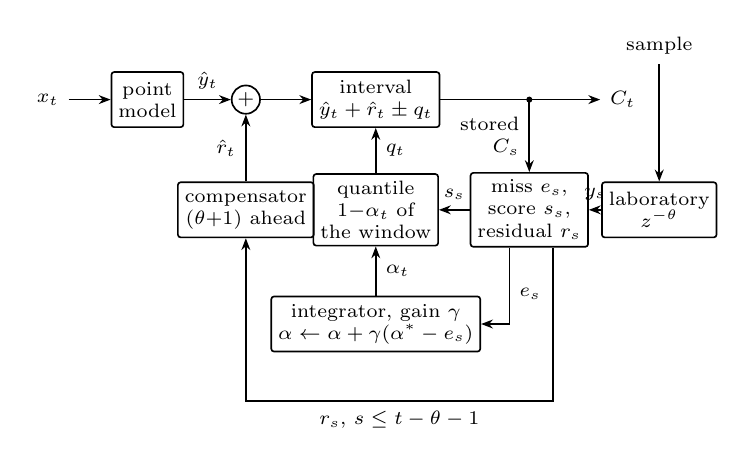
\begin{tikzpicture}[
    font=\scriptsize, >={Stealth[length=1.5mm]}, semithick,
    blk/.style={draw, rounded corners=1pt, align=center, inner sep=2.5pt,
      minimum height=7mm},
    sum/.style={draw, circle, inner sep=0pt, minimum size=3.6mm}]
  \node[blk] (model) at (0,0) {point\\model};
  \node[sum] (sum) at (1.25,0) {$+$};
  \node[blk] (int) at (2.9,0) {interval\\$\hat y_t + \hat r_t \pm q_t$};
  \node[blk] (comp) at (1.25,-1.4) {compensator\\$(\theta{+}1)$ ahead};
  \node[blk] (quant) at (2.9,-1.4) {quantile\\$1{-}\alpha_t$ of\\the window};
  \node[blk] (miss) at (4.85,-1.4) {miss $e_s$,\\score $s_s$,\\residual $r_s$};
  \node[blk] (lab) at (6.5,-1.4) {laboratory\\$z^{-\theta}$};
  \node[blk] (integ) at (2.9,-2.85) {integrator, gain $\gamma$\\$\alpha \leftarrow \alpha + \gamma(\alpha^\ast - e_s)$};
  \draw[->] (-1.0,0) node[left] {$x_t$} -- (model);
  \draw[->] (model) -- node[above] {$\hat y_t$} (sum);
  \draw[->] (sum) -- (int);
  \draw[->] (int.east) -- (5.75,0) node[right] {$C_t$};
  \draw[->] (4.85,0) -- node[left, align=right] {stored\\$C_s$} (miss.north);
  \draw[->] (6.5,0.45) node[above] {sample} -- (lab.north);
  \draw[->] (lab) -- node[above] {$y_s$} (miss);
  \draw[->] (miss) -- node[above] {$s_s$} (quant);
  \draw[->] (quant) -- node[right] {$q_t$} (int);
  \draw[->] (integ) -- node[right] {$\alpha_t$} (quant);
  \draw[->] ([xshift=-2.5mm]miss.south) |- node[pos=0.3, right] {$e_s$} (integ.east);
  \draw[->] ([xshift=3mm]miss.south) -- ++(0,-1.95) -| node[pos=0.25, below] {$r_s$, $s \le t-\theta-1$} (comp.south);
  \draw[->] (comp) -- node[left] {$\hat r_t$} (sum);
  \fill (4.85,0) circle (1.1pt);
\end{tikzpicture}
\caption{The calibrated soft sensor with delayed labels. The interval is centred on the point
prediction plus the predicted residual $\hat r_t$ ($\hat r_t = 0$ without compensation,
Section~\ref{sec:remedies:comp}); its half-width is the conformal quantile at level
$1 - \alpha_t$ of the last $W$ scores. The label $y_s$ arrives $\theta$ updates after the interval
for sample $s$ was issued and moves the level one update later, through an integrator of gain
$\gamma$; its miss $e_s$ is judged against the stored interval $C_s$. The calibrator is an
integral loop with dead time $\theta$.}
\label{fig:block}
\end{figure}

\subsection{Documented delays}\label{sec:loop:delays}

Table~\ref{tab:delays} derives $\theta$ from documented delays for the two processes of the
study. In the debutanizer, the butane content of the bottoms is measured by a gas chromatograph
on the overhead of the downstream column, with a 15-min cycle and about 45~min from sample to
result \citep[Sec.~6.2]{fortuna2007}; the same book also gives 20 to 60~min
\citep[Sec.~5.5]{fortuna2007}, and 30 to 75~min is reported by \citet[p.~42]{siddharth2019}. The
book models the seven inputs of the public data set at 12-min updates (Sec.~6.2) but analyses a
recording of the same column at 6-min updates (Sec.~4.1), with outlier counts out of 2394 rows,
the public file's length; it does not say which applies, so $\theta = 3$ is primary and
$\theta = 7$ secondary. The Tennessee Eastman product analyzer has a sampling interval and a dead
time of 0.25~h \citep[Table~5]{downs1993}. The same delay gives a dead time of 4 at 3-min
updates and of 14 at 1-min updates, and of 0 if the calibrator updates only when a new analyzer
value appears: the faster the calibrator runs on held labels, the longer its dead time.

\begin{table}[t]
\centering\footnotesize
\caption{Dead time from documented delays: label age $a = \lceil D/\Delta u \rceil$ and
$\theta = a - 1$ (Eq.~\eqref{eq:theta}). Debutanizer: gas chromatograph with a 15-min cycle,
about 45~min \citep[Sec.~6.2]{fortuna2007}; the range combines 20 to 60~min
\citep[Sec.~5.5]{fortuna2007} and 30 to 75~min \citep[p.~42]{siddharth2019}; the book gives
12-min and 6-min updates without saying which fits the public data set. Tennessee Eastman:
product analyzer XMEAS(40) \citep[Table~5]{downs1993}; $D$ counts from the row whose inputs give
the prediction to the row in which the label is written (counted from the composition's capture,
a reading is one row older when it first appears). Primary cells in bold.}
\label{tab:delays}
\begin{tabular}{@{}llrrr@{}}
\toprule
Process & Delay $D$ & $\Delta u$ & $a$ & $\theta$ \\
\midrule
Debutanizer & about 45 min & 12 min & 4 & \textbf{3} \\
            & about 45 min & 6 min & 8 & 7 \\
            & 20 to 75 min & 12 or 6 min & 2 to 13 & 1 to 12 \\
Tennessee Eastman & 0.25 h & 3 min & 5 & \textbf{4} \\
                  & 0.25 h & 1 min & 15 & 14 \\
                  & 0.25 h & per new value & 1 & 0 \\
\bottomrule
\end{tabular}
\end{table}

\subsection{What is measured}\label{sec:loop:metrics}

The primary measure is the uninformative share $U$: the share of issued intervals that are
infinite or wider than the range of $y$ over the calibration data. An operator cannot act on
such an interval, whatever the coverage figure says. Marginal coverage, the share of labelled
intervals that contain $y$, is reported with its Wilson 95\,\% interval \citep{wilson1927};
widths by the median, the 90th and the 99th percentiles of the finite widths; local behaviour by
the worst rolling coverage, the minimum coverage over 100 consecutive intervals. The persistence
of the misses is measured by the lag-1 autocorrelation of the miss indicator $e$, the mean length
of a run of consecutive misses, and the integrated autocorrelation time (IACT),
$1 + 2\sum_{k \ge 1} \rho_e(k)$, summed over an automatic window (Section~\ref{sec:study}). The
IACT is the factor by which serial correlation inflates the variance of a mean of misses, and so
of the level that Eq.~\eqref{eq:loop} integrates from them.

\section{Analysis and remedies}\label{sec:analysis}

\subsection{A stability limit that falls with the delay}\label{sec:analysis:p1}

Linearise Eq.~\eqref{eq:loop} about the target. If the window's scores represent the score
distribution, an interval issued at level $\alpha$ misses with probability close to $\alpha$, so
the level error $\varepsilon_t = \alpha_t - \alpha^\ast$ obeys
\begin{equation}
  \varepsilon_{t+1} = \varepsilon_t - \gamma\,(\varepsilon_{t-\theta} + \eta_{t-\theta}),
  \label{eq:linear}
\end{equation}
where $\eta_t = e_t - \mathrm{E}[e_t \mid \alpha_t]$ is the miss noise. The calibrator is an
integral controller of gain $\gamma$ acting through a dead time of $\theta$ updates. Its
characteristic polynomial $z^{\theta+1} - z^{\theta} + \gamma$ has all its roots inside the unit
circle if and only if
\begin{equation}
  0 < \gamma < \gamma_{\mathrm{crit}}(\theta) = 2\sin\!\left(\frac{\pi}{4\theta+2}\right)
  = 2\cos\!\left(\frac{\theta\pi}{2\theta+1}\right),
  \label{eq:gammacrit}
\end{equation}
the stability condition of the difference-delay equation
$\varepsilon_{t+1} - \varepsilon_t + \gamma\varepsilon_{t-\theta} = 0$, which \citet{levin1976} state
in the second form. The limit is 2 without delay, 1 at $\theta = 1$, 0.347 at $\theta = 4$ and
0.108 at $\theta = 14$: like any integral loop with dead time, the delayed calibrator tolerates
less gain the longer the dead time. Delayed-feedback versions of the recursion have been run
without this analysis \citep{dixit2023,szabadvary2024}, and \citet{szabadvary2024} suggests
larger steps the further ahead one predicts; the stable range shrinks with the delay instead.

\subsection{Why marginal coverage cannot see it}\label{sec:analysis:p2}

The level starts at $\alpha^\ast \in (0, 1)$. A miss needs a finite interval, issued at a level
of at least $1/(W+1) > 0$; a hit of a positive score needs a nonzero half-width, issued at a level
below 1. Each label moves the level by less than $\gamma$, $\theta + 1$ updates after its interval
was issued, so the level can pass 0 or 1 by at most $\theta + 1$ such steps: for positive scores
it stays in $[-\gamma(\theta+1),\, 1 + \gamma(\theta+1)]$. Summed over the $T$ labels that have
fed the loop, Eq.~\eqref{eq:loop} gives $\gamma\sum_s (\alpha^\ast - e_s)$ as the change in level,
and the realised miscoverage satisfies
\begin{equation}
  \Bigl|\, \frac{1}{T}\sum_s e_s - \alpha^\ast \Bigr| \le \frac{1 + 2\gamma(\theta+1)}{\gamma T}.
  \label{eq:p2}
\end{equation}
Marginal coverage therefore converges to $1 - \alpha^\ast$ by construction, however many of the
intervals were infinite: an infinite interval counts as a hit and pushes the level back up.
Eq.~\eqref{eq:p2} extends the argument of \citet{gibbs2021aci} to the delayed single-state loop.
It is the level-space analogue of the bound of \citet[Cor.~1]{wang2024acmcp} for the same
recursion in quantile space; related bounds grow with the delay \citep[Thm.~2]{ding2025multiqt} or
with the batch size \citep[Thm.~4.1]{areces2025}, and schemes of interleaved, delay-free chains are
bounded by \citet{elhalabi2026} and \citet{cherenson2026}. Marginal
coverage hides clustered misses \citep{retzlaff2025} and says nothing about the next interval
\citep{li2026breaks}; a coverage of 0.90 says nothing about how many intervals were usable, so $U$
has to be reported beside it.

\subsection{Why persistence matters}\label{sec:analysis:persistence}

For residuals without serial correlation the miss noise in Eq.~\eqref{eq:linear} is white, with
variance $\alpha^\ast(1-\alpha^\ast)$, and the standard deviation of the level follows from the
loop's frequency response,
\begin{equation}
  \sigma_\alpha^2 = \alpha^\ast(1-\alpha^\ast)\,\frac{1}{2\pi}\int_{-\pi}^{\pi}
  \bigl|H(e^{\mathrm{i}\omega})\bigr|^2\,\mathrm{d}\omega,
  \label{eq:noisegain}
\end{equation}
where $H(z) = -\gamma/(z^{\theta+1} - z^{\theta} + \gamma)$ carries the miss noise to the level.
Even for uncorrelated residuals it is approximate: in simulations before the study it was within
6\,\% of the measured spread for $\gamma \ge 0.02$ but 22 to 38\,\% high at $\gamma = 0.005$, where
the window adds feedback of its own (supplementary material). Intervals become
infinite when the level falls below $1/(W+1) \approx 0$, so a Gaussian level predicts an infinite
share $\Phi(-\alpha^\ast/\sigma_\alpha)$, a tail that is unreliable even then. The largest step
that keeps it below $\varepsilon = 1\,\%$, searched below $0.8\gamma_{\mathrm{crit}}$, is the
white-noise rule.

Process residuals are persistent. Misses then come in runs, and $\eta$ is coloured, with its
power at the low frequencies that the loop passes with unit gain ($|H(1)| = 1$). The white-noise
model underestimates how far the level wanders: on the study's data it underestimated
$\sigma_\alpha$ by 33 to 73\,\% in all 47 cells checked, and the infinite share by 81 to 100\,\% in
the 24 cells that had infinite intervals (Section~\ref{sec:results:tuning}). Without delay,
\citet{zaffran2022} found on AR(1) residuals that very large steps make the loop less stable and
produce numerous infinite intervals; with labels admitted a year late, an adaptive conformal loop
has been seen to overcorrect at a fixed step of 0.01 \citep{maligireddy2026}. With delay, the step
that holds a budget is set by persistence, far below the stability limit
(Fig.~\ref{fig:stability}): all 46 steps that the replay of Section~\ref{sec:remedies:replay}
selected on the study's calibration data lie at or below 2.8\,\% of $\gamma_{\mathrm{crit}}$. The
white-noise rule lies above every one of them for $\theta \ge 1$, at 2.5 to 9.5 times the largest
step selected at each $\theta$ (it holds the infinite share at $\varepsilon$, the replay holds
$U$ at $\varepsilon/2$). The step has to be chosen on the residuals themselves.

\begin{figure}[t]
\centering
\includegraphics[width=\columnwidth]{n1_stability.pdf}
\caption{Step sizes against the stability limit. Lines: the limit $\gamma_{\mathrm{crit}}(\theta)$
of Eq.~\eqref{eq:gammacrit}, the replay's cap $0.8\gamma_{\mathrm{crit}}$, and the white-noise rule
(Section~\ref{sec:analysis:persistence}, $\varepsilon = 1\,\%$). Markers: the step sizes selected by
replay to $\varepsilon/2$ on the study's calibration data (Section~\ref{sec:remedies:replay}),
uncompensated and compensated, per operating point for the Tennessee Eastman arms T1 (3-min
updates) and T2 (1-min updates), and for the debutanizer; markers are offset around their
$\theta$. Two uncompensated T2 tunings (operating point 1, $\theta = 4$ and 14) were infeasible and
run at 0.001.}
\label{fig:stability}
\end{figure}

\subsection{Remedy 1: tune the step by replaying history through the delayed loop}
\label{sec:remedies:replay}

Replay the calibration residuals through Eq.~\eqref{eq:loop} at the plant's $\theta$, for each
step on a grid from 0.001 to 0.1 (13 values) in ascending order, stopping at
$0.8\gamma_{\mathrm{crit}}(\theta)$, and select the largest step below the first whose replayed $U$
exceeds a target. The study targets $\varepsilon/2 = 0.5\,\%$ for a budget of $2\varepsilon =
2\,\%$, a margin fixed by a power analysis on simulated residuals before the protocol was frozen
(Section~\ref{sec:study}). If even 0.001 exceeds the target, the loop runs at 0.001, flagged
infeasible. Tuning on history that ignores the delay is the same rule at $\theta = 0$; the study
runs it to the target $\varepsilon$ and calls it delay-blind.

\subsection{Remedy 2: compensate the predictable residual first}\label{sec:remedies:comp}

Process control meets dead time by predicting the disturbance over it: a minimum-variance
controller removes the part of the disturbance that is predictable $\theta + 1$ steps ahead and
leaves only the $(\theta+1)$-step prediction error \citep{astrom1970}. Forecasting the score or
the residual at the label horizon ahead of a conformal loop is not new: conformal PID control
forecasts the score quantile \citep{angelopoulos2023pid}, and AcMCP adds a forecast of the
multi-step error to a delayed loop \citep{wang2024acmcp}, whose authors also compare that loop
with and without the forecast on coverage over rolling windows. That comparison fired the
literature rule of this paper's pre-registration (F4) before any data, and the claim was
narrowed: local coverage is reported here, not claimed. Compensation is treated here as dead-time
compensation of the loop. Applied to the sensor, the residual is predicted $\theta + 1$ updates
ahead from the labels in hand,
\begin{equation}
  \hat r_t = b_0 + \sum_{j=1}^{p} b_j\, r_{t-\theta-j},
  \label{eq:comp}
\end{equation}
the interval is centred on $\hat y_t + \hat r_t$, and the delayed loop calibrates only the
prediction error, through the score $s_t = |r_t - \hat r_t|$. The predictor is fitted by least
squares on the calibration segment, with $p$ chosen by the Bayesian information criterion from 1
to 10, and then stays fixed; apart from the last $\theta$ calibration labels, which a plant would
receive during the first $\theta$ evaluation updates, it sees labelled residuals only.
Compensation narrows the interval, because the window now holds prediction errors instead of
residuals. The narrowed claim, claim~2$'$, is that compensation also makes the miss process less
persistent and admits a larger step at the same budget; the study tests it on the Tennessee
Eastman process at $\theta = 4$ (Section~\ref{sec:results:persistence}).

\subsection{What compensation can buy, before deployment}\label{sec:remedies:p3}

Let $r$ be stationary and zero-mean, with autocorrelation $\rho$. The best linear predictor of
$r_t$ from $r_{t-\theta-1}, \dots, r_{t-\theta-p}$ leaves the fraction $1 - c^{\top}R^{-1}c$ of the
residual variance, with $c_j = \rho(\theta+j)$ and $R_{jk} = \rho(|j-k|)$. When the prediction
error and the residual share one standardised distribution, as Gaussian residuals do, the ratio
of compensated to uncompensated interval widths is
\begin{equation}
  \frac{w_{\mathrm{c}}}{w_{\mathrm{u}}} = \bigl(1 - c^{\top}R^{-1}c\bigr)^{1/2}.
  \label{eq:p3}
\end{equation}
The fraction cannot rise with $p$. Its limit is the $(\theta+1)$-step minimum-variance prediction
error, which \citet{harris1989} made the benchmark of control-loop performance assessment; no
linear predictor of the same labels does better. For AR(1) residuals with coefficient $\phi$ the
fraction is $1 - \phi^{2(\theta+1)}$ at every $p$: with $\phi = 0.9$, an immediate label
($\theta = 0$) leaves 44\,\% of the width and a dead time of 4 leaves 81\,\%. Eq.~\eqref{eq:p3}
needs only the autocorrelation of the calibration residuals, so the width that compensation can
buy can be predicted before deployment, at every analyzer delay; in the study the prediction
erred, on average, on the safe side in every case checked (Section~\ref{sec:results:p3}). Drawn
against the label age, it is an analyzer-speed chart that prices a faster or a closer analyzer
in interval width (Fig.~\ref{fig:speed}). Without delay, the gain from modelling past scores is
known to grow with their lag-1 autocorrelation \citep{areces2025}; Eq.~\eqref{eq:p3} makes the link
quantitative and delay-dependent. For other shapes the width ratio can differ from
Eq.~\eqref{eq:p3} (Section~\ref{sec:discussion}).

\begin{table*}[t]
\centering\footnotesize
\caption{The decided rules and their verdicts. Each rule was fixed with its threshold before any
result of the study existed (Section~\ref{sec:study}); a rule that fires removes or restricts the
claim it guards, and one that does not fire leaves it standing. The literature rule F4 fired
before the data and narrowed the claim on compensation to claim~2$'$
(Section~\ref{sec:remedies:comp}). F2 fires if neither primary cell shows a rise in $U$
over $\theta = 0$ of at least 1 percentage point (pp) with a 97.5\,\% interval above 0, and
restricts the diagnosis to the cell that shows it; F3 fires if 0.90 lies outside the Wilson
interval where the rise is shown; F5a and F5b if the mean $U$ exceeds 2\,\%; F6 if the mean error
of the predicted width ratio lies outside $\pm 10$\,\%; F7 if a baseline is valid and either it is
narrower or the loop is not valid; F8 if the 95\,\% interval of the paired difference in IACT does not lie wholly
below 0, and its step-size statement needs a larger compensated step in at least two operating
points and a smaller one in none. F1 is secondary and decides nothing.}
\label{tab:rules}
\input{\figdir/n1_table_rules.tex}
\end{table*}

\section{Pre-registered study}\label{sec:study}

The design below, the rules of Table~\ref{tab:rules} with their thresholds, the analysis plan and
the baseline configurations were frozen in a public repository on 29 October 2026, before any
result of the study existed (Data and code availability). Stage A of the run read training and
calibration rows only: it fitted the point models and compensators, tuned every step size, configured the
baselines and recorded every predicted width ratio, and its records were committed and pushed
before stage B read an evaluation row. Stage B recomputed stage A's quantities from the same files
and passed all 1359 checks against them exactly before evaluating. One deviation was logged before
any result: the arm that updates once per analyzer value seeds its window with 40 labels instead
of 200, because its calibration hours hold only 160; no rule is decided on that arm. Claude
(Anthropic) assisted in writing the analysis code and in screening the literature; the code's
results are checked as above, and every screening verdict is recorded with its source in the
repository.

\subsection{Data and point models}\label{sec:study:data}

\emph{Tennessee Eastman process (TEP).} The plant of \citet{downs1993} was simulated with the closed-loop
Fortran code of Russell, Chiang and Braatz \citep{russell2000}, with the feed-composition,
feed-temperature and reaction-kinetics disturbances IDV(8), IDV(10) and IDV(13) active
throughout, at three operating points set by the reactor-feed composition loops: the base case of
\citet{downs1993} and two with more G in the product (G at about 53.8, 58.2 and 63.4~mol\,\%;
operating points 1 to 3, labelled mode 1 to 3 in the figures). Each run drew its random
numbers from its own MRG32k3a stream \citep{lecuyer1999}, because the simulator's generator loses
precision in double-precision arithmetic \citep{kitchin2026} and then cycles within 0.55 to
141~h (supplementary material). For each operating point, the first five streams in a fixed
order whose 100-h run did not shut down were kept (5 of 26 candidates survived at the first, 14 of
25 and 17 of 25 at the others), so the evidence is conditional on runs that stay within the
plant's limits. Rows are 60~s apart: hours 0--30 train the point model, 30--70 calibrate and
70--100 evaluate. The target is the product G analysis, XMEAS(40). The point model is a ridge
regression on the 22 continuous measurements and 12 manipulated variables taken 15~min earlier,
its penalty chosen by fivefold cross-validation with the one-standard-error rule. One model per
run serves three arms that differ only in the calibrator: T1 updates every 3~min
($\theta = 0, 2, 4$), T2 every minute ($\theta = 0, 4, 14$) and T3 once per new analyzer value
($\theta = 0$). Gradient boosting on the same inputs checks the estimator class at T1.

\emph{Debutanizer.} The public data of \citet{fortuna2007} are one stream of 2394 rows. The butane
content is regressed on input $u_5$ 15 rows earlier by least squares on the first 1675 rows, whose
1660 residuals form the calibration segment; the other 719 rows are evaluated, at
$\theta = 0, 1, 3, 7$ and 12. The lag was chosen in earlier work on rows 0 to 2033, so for that one
choice the first 359 evaluated rows are not out of sample.

\begin{figure*}[t]
\centering
\includegraphics[width=\textwidth]{n1_diagnosis.pdf}
\caption{The diagnosis. Uninformative share $U$ (top) and coverage (bottom) against the dead time
$\theta$ for three ways of choosing the step: replay at the plant's $\theta$ to $\varepsilon/2$,
delay-blind tuning (replay at $\theta = 0$ to $\varepsilon$) and the white-noise rule
(Section~\ref{sec:analysis:persistence}); arms T1 (3-min updates; a, b) and T2 (1-min updates; c,
d), without and with compensation. Means over the 15 runs with 95\,\% $t$ intervals; markers are
offset around their $\theta$. Grey lines: the budget for $U$, 2\,\%, and the nominal coverage,
0.90. Coverage stays between 0.885 and 0.902 in every cell, while $U$ rises with $\theta$ under the two policies
that ignore the delay or the persistence.}
\label{fig:diagnosis}
\end{figure*}

\subsection{Cells, baselines and inference}\label{sec:study:cells}

A cell fixes the loop, the step-size policy, the pairing and the compensation; every contrast
varies one of them on a shared residual stream. The loops are the sequential loop of
Eq.~\eqref{eq:loop} (primary); split conformal, calibrated once (loop off); the level projected
onto $[0.01, 0.5]$; $\theta + 1$ interleaved delay-free chains \citep{elhalabi2026}; a
Smith-predictor form, in which the model $\mathrm{E}[e \mid \alpha] = \alpha$ swaps the miss rate
expected at the stored level for that at the current one; and decaying steps $c\,n^{-0.6}$
\citep{angelopoulos2024decay}. The policies are the fixed steps 0.005 \citep{gibbs2021aci} and
0.05, delay-blind tuning, replay to $\varepsilon$ and to $\varepsilon/2$, and the white-noise rule;
every loop is tuned by the same replay. The first 200 calibration scores seed the replay's window,
and every replayed update counts; on the Tennessee Eastman data the calibration segments of an
operating point's five runs are pooled, standing in for the longer history a plant would tune on.
Each run is evaluated from a window holding its last 200 calibration scores. Stored pairing is
primary; arrival pairing at the documented delay is the negative control.

Four baseline configurations get the same point model and only the labels in hand at issue.
Conformal PID control \citep{angelopoulos2023pid} runs with three scorecasters: quantile
regression on the three latest labelled scores, a linear form that \citet{areces2025} fit online;
the Theta model of the authors' code; and the compensator of Eq.~\eqref{eq:comp}, which gives it
the structure of AcMCP \citep{wang2024acmcp}. Its gains are tuned by the same replay to the same
target. SPCI \citep{xu2023spci} predicts the residual quantiles at horizon $\theta + 1$ with a
quantile random forest, without coverage feedback. Each follows its paper and, where the paper is
silent, the authors' code, with departures, each with its reason, listed in Appendix A of the
pre-registration (among them a warm start from the loop's seed rows and an unpenalised quantile
regression).

The 15 runs are independent replications: means carry 95\,\% $t$ intervals over the runs,
contrasts are paired by run, and pooled coverage carries a Wilson interval; the five runs of an
operating point share a tuned step, a dependence the $t$ intervals ignore. On the single
debutanizer stream, intervals come from a circular block bootstrap \citep{politis1992} of the
per-step indicators, with 2000 resamples, blocks of $\max(25, \lceil 2\,\mathrm{IACT}\rceil)$
steps and the same blocks for both arms of a contrast. The IACT is summed over the automatic
window of \citet{sokal1997} with $c = 5$. The rules are decided on the primary cells: F2 and F3 on
the uncompensated delay-blind loop, against $\theta = 0$ on the same stream, at T1, $\theta = 4$
and at the debutanizer's $\theta = 3$; F5 to F8 at T1, $\theta = 4$ (Table~\ref{tab:rules}).
Every other cell is descriptive. A power analysis on simulated AR(1) residuals set the margins: a
loop tuned to $\varepsilon$ met it on average, but its 15-run mean exceeded it in 21 to 38\,\% of
200 studies; tuned to $\varepsilon/2$, it exceeded the budget of $2\varepsilon$ in at most
4\,\%. F2 had a power of 0.91 to 0.99 in the Tennessee Eastman design, against 0.095 to 0.12 on
one stream of the debutanizer's length.


\section{Results}\label{sec:results}

Table~\ref{tab:rules} gives the verdicts: the diagnosis is shown on the Tennessee Eastman process
and not on the debutanizer, F1 fires, and no other rule decided on the data fires (the literature
rule F4 fired before the data; Section~\ref{sec:remedies:comp}). This section reports the cells
behind the verdicts; the supplementary material lists every cell and contrast.

\begin{table*}[t]
\centering\footnotesize
\caption{Seven cells at T1, $\theta = 4$: means over the 15 runs. Loop off: split conformal,
calibrated once. Median width: the run median of the finite interval widths, in mol\,\%; worst
rolling coverage: the minimum over 100 consecutive intervals; sd($\alpha$): the standard deviation
of the level; IACT of the misses. Last rows: the paired difference, compensated minus
uncompensated, under replay to $\varepsilon/2$, with its 95\,\% $t$ interval (coverages as
fractions).}
\label{tab:t1cells}
\input{\figdir/n1_table_t1_cells.tex}
\end{table*}

\begin{table*}[t]
\centering\footnotesize
\caption{The compensated loop (replay to $\varepsilon/2$) against four baseline configurations at
T1, $\theta = 4$: means over the 15 runs. Valid: mean $U$ at most 2\,\% and mean coverage within
2 points of 0.90. F7 width: the run median over all issued intervals, infinite ones included,
in mol\,\%.
Coverage-matched width change: each run's baseline width scaled to the loop's coverage in that run
by the ratio of Gaussian quantiles, against the loop's width; in brackets, the runs in which the
baseline is narrower. F7 fires if a valid baseline is at least 5\,\% narrower on average and
narrower in at least 12 of the 15 runs.}
\label{tab:baselines}
\input{\figdir/n1_table_baselines.tex}
\end{table*}

\subsection{The diagnosis on the Tennessee Eastman process}\label{sec:results:diagnosis}

With the step tuned on history that ignores the delay, the uninformative share rises with the
dead time (Fig.~\ref{fig:diagnosis}). In the primary cell, T1 at $\theta = 4$, 6.89\,\% of the
intervals were uninformative, 6.04 points more than at $\theta = 0$ on the same runs (97.5\,\%
CI 3.41 to 8.68; higher in 13 of 15 runs), while coverage read 0.8974 (8077 of 9000 labels;
Wilson 95\,\% interval 0.8910 to 0.9035, which contains 0.90): F2 is shown and F3 does not fire.
The rise grows with the dead time: 3.00 points at $\theta = 2$ and, in T2, 3.07 points at
$\theta = 4$ and 11.46 points at $\theta = 14$ (97.5\,\% CI 5.23 to 17.68), at coverages of 0.890 to
0.898; at T2 the pooled Wilson intervals lie just below 0.90 at every dead time, $\theta = 0$
included (pooled coverage 0.8903 to 0.8955). Compensation does not rescue a delay-blind step. At T2, $\theta = 14$,
the compensated loop issued 20.54\,\% uninformative intervals against 11.74\,\% without
compensation: the replay at $\theta = 0$ chose larger steps for the compensated residuals (0.010 to
0.015, against 0.001 to 0.010), and at $\theta = 14$ those steps issued more uninformative
intervals.

\begin{figure*}[t]
\centering
\includegraphics[width=\textwidth]{n1_speed_chart.pdf}
\caption{The analyzer-speed chart: width ratio, compensated over uncompensated, against the label
age $a = \theta + 1$ updates, in minutes for the Tennessee Eastman arms (left) and in samples for
the debutanizer (right). Open markers: predicted by Eq.~\eqref{eq:p3} from each run's calibration
residuals before the evaluation rows were read; filled markers: measured, as the ratio of the 0.90
quantiles of the evaluation scores, with 95\,\% $t$ intervals over the 15 runs (the debutanizer is
one stream). T3 updates once per analyzer value. Every measured ratio lies below its prediction.}
\label{fig:speed}
\end{figure*}

\subsection{Tuning}\label{sec:results:tuning}

Replay at the plant's dead time held the budget. At T1, $\theta = 4$, the uncompensated loop tuned
to $\varepsilon/2$ issued 0.30\,\% uninformative intervals (F5a; budget 2\,\%; two runs above
zero, at 3.67 and 0.83\,\%) at a coverage of 0.8926, and across the T1 and T2 cells the replay
kept the mean $U$ at or below 0.47\,\%, compensated or not (Fig.~\ref{fig:diagnosis}). Nine tunings, all at
T2's first operating point without compensation, were infeasible and ran at 0.001. The two
policies that each ignore one property of the loop did not hold the budget: against the replay,
delay-blind tuning added 6.59 points of $U$ (CI 4.18 to 9.00) and the white-noise rule 17.89
points (CI 15.04 to 20.74), both at nominal coverage. Their larger steps adapt faster locally,
with worst rolling coverage 5.0 and 8.3 points above the replay's 0.731 (Table~\ref{tab:t1cells}).
The white-noise model behind the rule failed as Section~\ref{sec:analysis:persistence} expects: it
underestimated $\sigma_\alpha$ by 33 to 73\,\% in all 47 uncompensated cells at the documented
dead times, and the infinite share by 81 to 100\,\% in the 24 cells that had infinite intervals
(F1 fires); with compensation it was off by more than 25\,\% in 40 of 41 cells. Fixed steps did not
hold the budget everywhere. The step of \citet{gibbs2021aci}, 0.005, held the budget at T1 but not at T2 (2.64\,\%
at $\theta = 4$ and 9.71\,\% at $\theta = 14$, uncompensated), and 0.05 gave 13 to 50\,\% in every
T1 and T2 cell with $\theta \ge 2$. Of the comparison loops tuned by the same replay, the interleaved chains, the
Smith-predictor form and decaying steps held the budget at T1, $\theta = 4$ ($U \le 0.48\,\%$,
coverage 0.891 to 0.897); projecting the level onto $[0.01, 0.5]$ removed the infinite intervals
but under-covered (0.858, and 0.841 with compensation).

\begin{figure*}[t]
\centering
\includegraphics[width=\textwidth]{n1_persistence.pdf}
\caption{Persistence and the step at T1, $\theta = 4$. (a) IACT of the open-loop misses ($\gamma =
0$, the window still rolling), per run, without and with compensation; grey lines join the runs,
large markers are means with 95\,\% $t$ intervals. (b) The step selected by replay to
$\varepsilon/2$ per operating point, without and with compensation.}
\label{fig:persistence}
\end{figure*}

\subsection{Compensation}\label{sec:results:comp}

Compensation narrowed the intervals at the same budget. At T1, $\theta = 4$, the compensated loop
tuned to $\varepsilon/2$ issued 0.18\,\% uninformative intervals (F5b; two runs above zero, at 0.83
and 1.83\,\%), and its run-median width was 0.461~mol\,\% smaller than without compensation (CI
0.200 to 0.723), 17.8\,\% of the uncompensated 2.586 (CI 7.7 to 28.0\,\%), at a coverage of 0.8961
against 0.8926 (Table~\ref{tab:t1cells}). Its worst rolling coverage was 6.53 points higher (CI
1.84 to 11.22; reported, not claimed, as Section~\ref{sec:remedies:comp} explains), and its misses
less persistent (IACT 3.97 against 7.84). On this plant, where
split conformal itself covered 0.900, the loop added nothing measurable to compensated split
conformal: $U$ $+0.18$ points, coverage $-0.37$ points (CI $-2.11$ to $+1.38$), width $+0.023$ (CI
$-0.102$ to $+0.149$) and worst rolling coverage $+2.53$ points (CI $-0.36$ to $+5.43$).
Section~\ref{sec:results:debutanizer} shows a stream where the loop raised coverage, by amounts
whose 95\,\% intervals just include 0. The negative control shows that the bookkeeping matters:
against stored pairing, arrival pairing (uncompensated, replay to $\varepsilon/2$) lowered coverage
by 0.64 points (CI 0.38 to 0.91) and the worst rolling coverage by 1.07 points (CI 0.03 to
2.10).

\begin{figure*}[t]
\centering
\includegraphics[width=\textwidth]{n1_debutanizer.pdf}
\caption{The debutanizer at $\theta = 3$: coverage over the last 100 evaluation rows for the
delayed loop (replay to $\varepsilon/2$) and for split conformal, (a) without and (b) with
compensation; the legend gives the coverage over all 719 evaluation rows. Grey line: the nominal
coverage, 0.90.}
\label{fig:debutanizer}
\end{figure*}

\subsection{Baselines}\label{sec:results:baselines}

No baseline was both valid and narrower (F7 does not fire; Table~\ref{tab:baselines}). All three
conformal PID configurations were valid. At coverage matched in each run, the matched scorecaster,
which shares the compensator, came within 1.5\,\% of the loop (narrower in 8 of 15 runs;
difference $-0.031$, CI $-0.093$ to $+0.031$); the quantile-regression scorecaster was 1.6\,\% wider
and the Theta scorecaster 17.7\,\% wider. SPCI under-covered (0.8673) and is not valid. The
delayed loop with the compensator thus matched the best conformal PID configuration with one
state and one tuned step, against three tuned constants. The PID-guided soft sensor of
\citet{meng2026}, whose update is a conformal PID variant without delay handling, is represented
here by conformal PID itself. On
the debutanizer at $\theta = 3$, the matched configuration covered 0.9013 at a width of 0.192,
against the loop's 0.8999 and 0.189.

\subsection{Predicting the width}\label{sec:results:p3}

Eq.~\eqref{eq:p3}, evaluated on each run's calibration residuals before any evaluation row was
read, predicted a mean width ratio of 0.880 at T1, $\theta = 4$; the ratio measured on the
evaluation rows was 0.835. The mean error over the runs, $-4.9$\,\% (CI $-13.2$ to $+3.5$\,\%),
lies inside the $\pm 10$\,\% of F6, although single runs erred from $-27.5$ to $+16.0$\,\%. In all
15 cells of the chart, the 12 drawn in Fig.~\ref{fig:speed} and the three of the gradient-boosting
arm, the measured ratio lies below the prediction on average, by 0.2 to 7.1\,\% in eight cells and
by 18 to 44\,\% in seven, at the shortest label ages (T1 and T2 at $\theta = 0$) and on the
debutanizer: on average, compensation bought at least the predicted narrowing. Read along the label age, the chart prices the analyzer: on the Tennessee Eastman
process, a label 3~min old instead of 15~min would let compensation cut the width to 0.47 of the
uncompensated width instead of 0.88 (predicted; measured 0.39 and 0.84).

\subsection{Persistence and the step}\label{sec:results:persistence}

F8's gate passed (mean predicted ratio 0.880, at most 0.95), and compensation made the misses less
persistent. The IACT of the open-loop misses ($\gamma = 0$, the window still rolling) fell by 4.69
(CI 1.55 to 7.82) and was lower in 12 of 15 runs (Fig.~\ref{fig:persistence}a); their lag-1
autocorrelation fell by 0.058 (CI 0.013 to 0.103) and the mean run of consecutive misses by 0.64
(CI 0.14 to 1.14), with the miss rate 1.0 point lower (CI $-0.2$ to $+2.2$). With compensation the
replay held the budget at a larger step, as claim~2$'$ states: 0.007 at all three operating points,
against 0.003, 0.003 and 0.007 without (larger at two, equal at the third;
Fig.~\ref{fig:persistence}b). The IACT fell in every arm, by 0.65 (T3) to 13.43 (T2,
$\theta = 0$), and on the debutanizer at $\theta = 3$ it fell from 24.7 to 5.2 while the replay's
step rose from 0.002 to 0.010.

\subsection{The debutanizer}\label{sec:results:debutanizer}

On the debutanizer the delay did not raise $U$ at the primary and secondary dead times: under
delay-blind tuning $U$ was 0 at $\theta = 0$, 1, 3 and 7, so F2 is not shown there and the
diagnosis is restricted to the simulated plant. At $\theta = 12$, the end of the documented range, $U$ rose by
5.42 points (97.5\,\% CI 0.00 to 18.36; 11 blocks), not shown either; F2's power on one stream of
this length was about 0.1 (Section~\ref{sec:study}). The stream showed something else. Split
conformal covered 0.7497, and its coverage over 100 rows fell to 0.06 late in the stream
(Fig.~\ref{fig:debutanizer}a), which suggests, without testing it, that the evaluation rows
differ from the training rows. Uncompensated, the delayed loop covered 0.8651 at $\theta = 3$,
11.5 points more than split conformal (CI $-0.1$ to $+27.3$), but stayed below 0.90 at every dead
time (0.844 to 0.878; 0.865 to 0.878 under delay-blind tuning). Compensated, it covered 0.8999 at a width of 0.189, against 0.8762 for
compensated split conformal ($+2.4$ points, CI $-0.7$ to $+5.3$), and 3.5 points more than without
compensation (CI $-3.8$ to $+11.4$) at 55\,\% of the width. The white-noise rule issued 22.53\,\%
uninformative intervals here.

\subsection{Robustness}\label{sec:results:robustness}

The diagnosis and the remedies held with gradient boosting as the point model: at T1, $\theta =
4$, F2's rise was 3.71 points (97.5\,\% CI 0.90 to 6.52), the replay held $U$ at 1.39\,\% without and
0.47\,\% with compensation, Eq.~\eqref{eq:p3} erred by $-0.2$\,\%, and compensation lowered the
IACT by 4.84. At T2's faster cadence the replay held $U$ at or below 0.47\,\%, and
Eq.~\eqref{eq:p3} erred by $-4.0$ and $-5.2$\,\% at $\theta = 4$ and 14 but by $-44.2$\,\% at
$\theta = 0$, on the safe side. At T3, which has no dead time, $U$ was 0.28 and 0.33\,\%,
Eq.~\eqref{eq:p3} erred by $-3.5$\,\%, and compensation still lowered the IACT, by 0.65 (CI 0.17 to
1.14), though its step was not larger at every operating point.

\section{Discussion}\label{sec:discussion}

For an engineer who sizes the interval of a soft sensor whose labels arrive late, the results
reduce to five rules.
\begin{enumerate}\setlength{\itemsep}{0pt}
\item Do not tune the step on history that ignores the delay, or by the rule for uncorrelated
residuals. On the simulated plant they left 6.9 and 18.2\,\% of the intervals uninformative
against a 2\,\% budget, at coverages of 0.897 and 0.899, so report $U$ beside the coverage.
\item Tune the step by replaying the calibration residuals through the delayed loop at the plant's
dead time; the step it chooses lies far below the stability limit.
\item Compensate the predictable part of the residual first: at the same budget the interval was
18\,\% narrower, its misses less persistent, and a larger step held the budget.
\item Before choosing or moving an analyzer, read the width that compensation would buy off the
autocorrelation of the calibration residuals (Eq.~\eqref{eq:p3}); on average, the gain was never
smaller than predicted.
\item Where the evaluation data resemble the calibration data, compensated split conformal may be
enough. Where they seem not to, as on the debutanizer stream (split conformal 0.750), the loop raised
the coverage to 0.865 and, compensated, to 0.900, against 0.876 for compensated split conformal
(Fig.~\ref{fig:debutanizer}); the 95\,\% block-bootstrap intervals of both gains include 0.
\end{enumerate}

\emph{Why the width prediction errs on the safe side.} Eq.~\eqref{eq:p3} assumes that the
compensated and uncompensated scores share one standardised shape. With other shapes the width
ratio can differ from the ratio of standard deviations: for AR(1) residuals with $\phi = 0.9$ and
uniform or $t_5$ innovations, simulated over 2 million steps before the study, the width ratio at
one step ahead lay 4.2 to 5.5\,\% below it, the same sign and size as the errors at the longer
label ages here (0.2 to 5.4\,\%). The larger errors (18 to 44\,\%) suggest two further sources,
neither tested here. At the shortest label ages on the Tennessee Eastman process the analyzer holds
each reading, with its noise, for 0.25~h, so the residual one update ahead is mostly predictable and
its prediction error far from Gaussian, a stronger shape effect than the simulated one. On the
debutanizer the prediction uses the calibration residuals, and a slow shift in the evaluation rows
widens the uncompensated interval, which must cover it, more than the compensated one, whose
predictor follows it; the split-conformal coverage of 0.750 points to such a shift.

\emph{Limits.} The diagnosis rests on a simulator: the Tennessee Eastman runs share one plant model
and three operating points, come from the streams that did not shut down (36 of 76 candidates),
and share a tuned step within each operating point. The debutanizer is one stream, on which F2 had a
power of about 0.1. The dead times follow from documented delays through a timing convention
(Table~\ref{tab:delays}), which a plant must check against its own data historian. The ridge
penalty sat at the top of its grid in 10 of the 15 runs, so the point model may be
over-regularised; the gradient-boosting arm gave the same results on every rule computed for it.
The baselines were configured from their papers and code before the data, and other settings may
serve them better. Random and irregular
delays \citep{shardt2016,guo2014} were not studied.


\section{Conclusion}\label{sec:conclusion}

A conformal soft sensor recalibrated with late laboratory labels is an integral loop with dead
time. Its linearisation bounds the step by $2\sin(\pi/(4\theta+2))$, its marginal coverage
converges however many of its intervals are uninformative, and on persistent process residuals
the step that holds a budget lies far below the bound. In a pre-registered study on the Tennessee
Eastman process, a step tuned without the delay left 6.9\,\% of the intervals uninformative at
nominal coverage. Replaying the calibration residuals through the delayed loop held a 2\,\%
budget, and compensating the residual over the dead time narrowed the intervals by 18\,\% at the
same budget, made the misses less persistent and admitted a larger step; no baseline
configuration was both valid and narrower. The width ratio that compensation buys was predicted
from the calibration residuals' autocorrelation to within 5\,\% on average at four updates, and
the gain it implies was never overstated on average, so an engineer can price a faster or closer
analyzer before buying it. The diagnosis
did not appear on the debutanizer stream, where split conformal covered only 0.750 and the
compensated loop 0.900. Random and irregular delays, plant data with time-stamped laboratory
delays, and a step-size-free loop analysed under delay are the next steps.


\section*{Data and code availability}
The protocol, code and evidence are public. The IPIS repository
(\url{https://github.com/beebzy-droid/IPIS}) holds the pre-registration, frozen at tag
\texttt{n1-phase1-freeze} on 29 October 2026, the runner, the records of stages A and B and the
figure generators; a recomputation of the verdicts from the committed records of stages A and B
on a second platform agreed with the first to within a relative difference of
$1.3 \times 10^{-9}$. The 15 Tennessee Eastman runs and the repository's files for this
study at the submission tag are archived at Zenodo \citep{busico2026data}; the runs can also be
regenerated by the repository's script from the simulator of \citet{russell2000} (sources at
\url{https://github.com/camaramm/tennessee-eastman-profBraatz}, commit 0643318) and the recorded
random streams, and are checked against the SHA-256 digests in the records. The debutanizer data
are those of \citet{fortuna2007} and are not redistributed. The supplementary material
lists every cell and contrast of the study, the baseline configurations and the checks of
Section~\ref{sec:study}.

\section*{CRediT authorship contribution statement}
\textbf{Bien Don Busico:} Conceptualization, Methodology, Software, Validation, Formal analysis,
Investigation, Data curation, Writing -- original draft, Writing -- review \& editing,
Visualization, Project administration.

\section*{Funding}
This research did not receive any specific grant from funding agencies in the public, commercial,
or not-for-profit sectors.

\section*{Declaration of competing interest}
The author declares no competing financial interests or personal relationships that could have
influenced the work reported in this paper.

\section*{Declaration of generative AI and AI-assisted technologies in the manuscript preparation
process}
During the preparation of this work, the author used Claude (Anthropic) in order to draft and edit
the text, write and check the analysis code, and screen literature records. After using this
tool, the author reviewed and edited the content as needed and takes full responsibility for the
content of the published article.

\bibliographystyle{elsarticle-num-names}
\bibliography{references}

\end{document}
